\documentclass[serif,notheorems]{beamer}
\usetheme{Berlin}
\usecolortheme{seagull}
\usepackage[utf8]{inputenc}
\usepackage[T1]{fontenc}
\usepackage{csvsimple}
\usepackage{graphicx}
\usepackage{verbatim}
\usepackage{sansmathaccent}
\pdfmapfile{+sansmathaccent.map}
\usepackage{amsmath,mathtools}

% immmagini
\graphicspath{ {./img/} } % Path relative to the main .tex file 
\usepackage[labelformat=empty]{caption}

% per inserire immagini:
%\begin{figure}[H]
%\centering
%\includegraphics[scale=.8]{Images/EM on elliptic data %3.png}
%\caption{E-M on elliptic data, 3 clusters}
%\end{figure}

% STUTTURE FONDAMENTALI
% ipotesi
\newenvironment{ipotesi}%
{\quad\left|\quad\def\arraystretch{1.2}\begin{array}{@{}l@{}}}%
{\end{array}\right.}
% tesi
\newcommand{\tesi}[1]{\quad\left|\quad{#1}\right.}
% unico comando per ipotesi e tesi
\newcommand{\hpth}[2]
{
\begin{align*}
\quad
\text{Ipotesi}
&\begin{ipotesi}
#1
\end{ipotesi}\\
\text{Tesi}
&\begin{ipotesi}
#2
\end{ipotesi}
\end{align*}
}
% quando si vuole inserire l'idea della dimostrazione
\newcommand{\hpthdim}[3]
{
\begin{align*}
\quad
\text{Ipotesi}
&\begin{ipotesi} 
#1
\end{ipotesi}\\
\text{Tesi}
&\begin{ipotesi}
#2
\end{ipotesi}\\
\text{Dim}
&\begin{ipotesi}
#3
\end{ipotesi}
\end{align*}
}
% quando ci sono 2 tesi distinte
\newcommand{\hpthth}[3]
{
\begin{align*}
\quad
\text{Ipotesi}
&\begin{ipotesi} 
#1
\end{ipotesi}\\
\text{Tesi 1}
&\begin{ipotesi}
#2
\end{ipotesi}\\
\text{Tesi 2}
&\begin{ipotesi}
#3
\end{ipotesi}
\end{align*}
}
% teoremi, definizoni, dimostrazioni, osservazioni
\setbeamertemplate{theorems}[numbered] % to number
\theoremstyle{definition} % insert bellow all blocks you want in normal text
\newtheorem{theorem}{Teorema}[section] % to number according to section
\newtheorem{definition}{Definizione}[section] % to number according to section
\newtheorem*{idea}{Idea dimostrazione} % no numbered block
\theoremstyle{remark}
\newtheorem*{remark}{Osservazione}


% NOTAZIONE
% sistemi
\newenvironment{system}%
{\left\lbrace\begin{array}{@{}l@{}}}%
{\end{array}\right.}
% parte intera
\newcommand{\interior}[1]{\accentset{\circ}{#1}}
% norma
\newcommand\norm[1]{\left\lVert#1\right\rVert}
% absolute value
\newcommand\abs[1]{\left|#1\right|}


% FUNZIONAMENTO MATRICI
\makeatletter
\renewcommand*\env@matrix[1][*\c@MaxMatrixCols c]{%
  \hskip -\arraycolsep
  \let\@ifnextchar\new@ifnextchar
  \array{#1}}
\makeatother





\title{Il teorema di Cauchy-Kowalevski\\ e alcune sue conseguenze }
\author{Candidato: Alessandro Pedone,\\ Relatore: Prof. Maurizio Grasselli }
\institute{Politecnico di Milano}
\date{24 settembre 2024}

\begin{document}

\frame{\titlepage}
\begin{frame}
    \frametitle{Indice}
    \tableofcontents
\end{frame}


\section{Introduzione}

\begin{frame}
\frametitle{Sofya Vasilyevna Kovalevskaya (1850-1891)}
Diamo per nota la figura storica di Augustin-Louis Cauchy. 
Kowalevski è stata:
\begin{itemize}
\item una matematica russa allieva di Weierstrass
\item la \textbf{prima donna} a conseguire un dottorato (3 tesi risalenti al 1874) e a ottenere una cattedra in Europa (in matematica)
\end{itemize}
\end{frame}

\begin{frame}
Esistono diverse sue \textbf{rappresentazioni artistiche} sia in letteratura che nel cinema. Le più rilevanti sono:
\begin{itemize}
\item Una biografia accurata: \textit{Little Sparrow: A Portrait of Sophia Kovalevsky} (1983), Don H. Kennedy
\item Un racconto breve: \textit{Too Much Happiness} (2009), Alice Munro
\end{itemize}
\end{frame}

\begin{frame}
\frametitle{Il problema}
\begin{itemize}
\item Cerchiamo delle condizioni che garantiscano l'esistenza di una soluzione analitica di un sistema di EDP con condizioni di Cauchy.
\item Se la soluzione esiste, è unica?
\item Se esiste un'unica soluzione, essa dipende con continuità dal dato iniziale? (\textit{buona positura secondo Hadamard})
\item Ragioniamo su alcune ulteriori conseguenze.
\end{itemize}
\end{frame}


\section{Nozioni e strumenti}

\begin{frame}
\frametitle{Classificazione EDP}
\begin{table}
\renewcommand{\arraystretch}{2}
\begin{tabular}{l l} 
\hline \hline
 Lineare & $\sum_{|\alpha |\leq k} a_\alpha \, D^\alpha u = f$ \\
 \hline
 \vspace{-2mm}
 Quasi-lineare & $\sum_{|\alpha |= k} a_\alpha (x,D^\beta u) \, D^\alpha u +  a_0(x,D^\beta u)= f,$\\
 & $\quad |\beta |<k $ \\
 \hline
 Non-lineare & $F(x,D^\alpha u)=0, \quad |\alpha | \leq k$ \\
 \hline
 In forma normale & $D_{t}^k u = G(x,t, D^\alpha_x D^j_t u), \, |\alpha |+j \leq k, \, j < k$ \\
 \hline \hline
\end{tabular}
\end{table}
\end{frame}

\begin{frame}
\frametitle{Nozioni e strumenti essenziali}
\begin{itemize}
\item Superfici caratteristiche
\item Metodo delle caratteristiche
\item Problemi di Cauchy
\item Serie di potenze
\end{itemize}
\end{frame}

\begin{frame}
\frametitle{Superfici caratteristiche}
$L$ operatore differenziale lineare.
\begin{definition}
Chiamiamo forma caratteristica di $L$
$$\chi_L(x,\xi)=\sum\limits_{|\alpha |= k} a_\alpha(x) \, \xi^\alpha \quad \text{con} \quad x,\xi \in \mathbb{R}^n$$
\end{definition}

\begin{definition}
Chiamiamo varietà caratteristica di $L$ in $x$ l'insieme
$$\text{char}_x (L)= \{ \xi \neq 0 : \chi_L(x,\xi)=0 \}$$
\end{definition}
\end{frame}

\begin{frame}
\begin{definition}
$\Gamma$ è una superficie caratteristica per $L$ in $x$ se $\nu(x) \in\text{char}_x (L)$.
\end{definition}
\begin{remark}
Caso di operatore del $1$° ordine: $A=(a_1,\ldots ,a_n)$ tangente a $\Gamma$.\\
Utile per generalizzazioni successive.
\end{remark}
\end{frame}

\begin{frame}
\frametitle{Significato}
\begin{itemize}
\item Se
$\xi \in \text{char}_x (L)$
$L$ non è ``propriamente'' di ordine $k$ in $x$ nella direzione $\xi$.
\vspace{5mm}
\item Assegnate su $\Gamma$ le derivate $D^i_\nu u \,(i<k)$ di una soluzione $u$, se
$\Gamma \text{ non è caratteristica }$
è possibile calcolare tutte le sue derivate parziali su $\Gamma$.
\end{itemize}
\end{frame}

\begin{frame}
\frametitle{Operatori quasi-lineari $1$° ordine}
\begin{itemize}
\item $\gamma: \mathbb{R}^{n-1}\rightarrow \mathbb{R}^n, \; \gamma = \gamma (s)$ parametrizzazione locale di $\Gamma$
\item $u = \phi$ su $\Gamma$ dato di Cauchy
\end{itemize}
\begin{definition}
$\Gamma$ si dice non caratteristica in $x_0=\gamma (s_0)$ se\\
\begin{equation*}
\det
\underbrace{
\left[
\begin{matrix}
D_{s_1}\gamma_1 & \cdots & D_{s_{n-1}}\gamma_1 \\
\vdots &  & \vdots \\
D_{s_1}\gamma_n & \cdots & D_{s_{n-1}}\gamma_n \\
\end{matrix}\;\right|}_{\text{span del piano tangente}} \,
\left.
\begin{matrix}
a_1(\gamma, \phi(\gamma))\\
\vdots\\
a_n(\gamma, \phi(\gamma))\\
\end{matrix}\right] (s_0) \neq 0
\end{equation*}
\end{definition}
\end{frame}

\begin{frame}
\frametitle{Metodo delle caratteristiche}
I problemi seguenti sono \textbf{equivalenti}.
\begin{equation} \label{edpquasilin}
\text{EDP : }
\begin{cases}
\sum a_j(x,u)D_{x_j} u = b(x,u)\\
u = \phi \text{ su } \Gamma
\end{cases} 
\end{equation}
\begin{equation}
\text{EDO : }
\begin{cases}
D_t \, x = A(x,y) \; \footnotemark \\
D_t \, y = b(x,y)\\ 
x(0)=x_0\\ 
y(0) = \phi (x_0) \quad \forall x_0 \in \Gamma
\end{cases} 
\end{equation}
dove $y = u(x)$ e $A(x,y)=[a_1(x,y),\ldots ,a_n(x,y)]$.
\footnotetext{le soluzioni $x$ vengono dette \textit{curve caratteristiche}}
\end{frame}

\begin{frame}
\begin{theorem}
\hpth{
\text{Problema \eqref{edpquasilin} } \\
a_j, \, b, \, \phi , \, \Gamma \in C^1\\
\Gamma \text{ non caratteristica}
}{
\exists ! \text{ soluzione } C^1 \text{ in un intorno di } \Gamma
}
\end{theorem}
{
La dimostrazione si svolge sfruttando il teorema di esistenza e unicità locale per EDO.
}
\end{frame}

\begin{frame}
\frametitle{Problema di Cauchy generale}
\begin{equation*}
\begin{cases}
F^*(x,D^\alpha u^*)=0 & |\alpha | \leq k, \, F^* \text{ almeno } C^1\\
D^j_\nu u^* = \phi_j^* & \text{su } \Gamma^* \text{ per }j<k 
\end{cases}
\end{equation*}
\end{frame}

\begin{frame}
\frametitle{Mappatura in $t=0$}
Detta $\gamma^*$ la parametrizzazione locale di $\Gamma^*$, applichiamo
$$\Phi (x) = 
\begin{bmatrix}[ccc|c]
x_1 & \cdots & x_{n-1} & x_n-\gamma^* (x_1,\ldots , x_{n-1})
\end{bmatrix}$$
\begin{figure}[H]
\centering
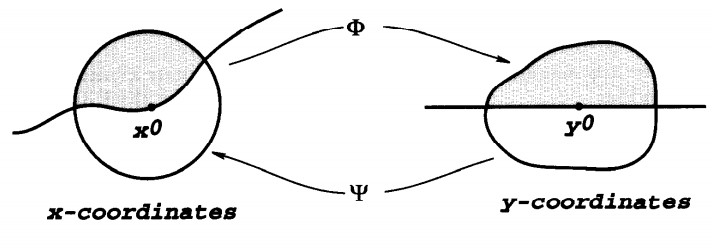
\includegraphics[scale=.35]{flatb}
\caption{\tiny{L. C. Evans, \textit{Partial Differential Equations}}}
\end{figure}
\end{frame}

\begin{frame}
\begin{enumerate}
\item Selezioniamo una variabile privilegiata e chiamiamola ``tempo'':
\begin{align*}
t & \leftarrow x_n \\
x & \leftarrow (x_1,\ldots , x_{n-1})
\end{align*}
\item Chiamiamo $\Gamma_0 = \{t=0\}$.
\item Indichiamo le derivate nel modo seguente: $D^\alpha_x D^j_t u$.
\item Otteniamo il problema ($u^*=u(\Phi)$):
\begin{equation*}
\begin{cases}
F(x,t, D^\alpha_x D^j_t u)=0 & |\alpha | +j \leq k\\
D^j_t u (x,0)= \phi_j(x) & \text{per }j<k 
\end{cases}
\end{equation*}
\end{enumerate}
\end{frame}

\begin{frame}
\frametitle{Superfici non caratteristiche in generale}
\begin{definition}
$\Gamma^*$ (o $\Gamma_0$) è non caratteristica se l'equazione su $\Gamma_0$ può essere riscritta in \textbf{forma normale} rispetto a $t$.
\end{definition}
\begin{remark}
Si dimostra che è coerente con le definizioni precedenti.
\end{remark}
\begin{remark}
\begin{itemize}
\item Caso lineare $\rightarrow$ condizione sui coefficienti.
\item Caso non-lineare $\rightarrow$ validità ipotesi teorema del Dini su $F$.
\end{itemize}
\end{remark}
\end{frame}


\begin{frame}
\frametitle{Metodo dei maggioranti}
\begin{definition}
Chiamiamo funzione maggiorante $$\mathcal{M}_{Cr}(x)=\frac{Cr}{r-(x_1+\ldots +x_n)}$$
\end{definition}
\begin{remark}
Per il teorema multinomiale se $|x|<r/n$ si ha che
$$\frac{Cr}{r-(x_1+\ldots +x_n)}=C \sum\limits_\alpha \frac{|\alpha |!}{\alpha ! \, r^{|\alpha |}} x^\alpha$$
\end{remark}
\end{frame}

\begin{frame}
\begin{theorem}[utilità del maggiorante]
\begin{equation*}
\begin{cases}
g_\alpha \geq |f_\alpha|\\
\sum g_\alpha x^\alpha \text{ ha raggio di conv. } R
\end{cases}
\implies 
\begin{array}{c}
\sum f_\alpha x^\alpha \\
\text{ha raggio almeno } R
\end{array}
\end{equation*}
\end{theorem}
In questo caso si scrive:  $\sum g_\alpha x^\alpha \gg \sum f_\alpha x^\alpha$.
\end{frame}

\begin{frame}
\begin{theorem}[costruzione del maggiorante]
$\sum f_\alpha x^\alpha$ ha raggio $R \implies \exists \, r<R, \, C>0$ tali che 
$$|f_\alpha | \leq C \frac{1}{r^{|\alpha |}} \leq C \frac{|\alpha |!}{\alpha ! \, r^{|\alpha |}}$$
\end{theorem}
\end{frame}


\section{Versione invariante}

\begin{frame}
\frametitle{Schema dell'approccio}
Seguendo l'ordine cronologico dei risultati procediamo per \textbf{generalizzazioni progressive}:
\begin{enumerate}
\item EDO
\item EDP quasi-lineari
\item EDP in forma normale
\end{enumerate}
\end{frame}


\begin{frame}
\frametitle{EDO}
\begin{theorem}
\hpth{
A \subseteq \mathbb{C}, \, B\subseteq \mathbb{C}^n \text{ aperti }\\
\Omega \subseteq A \text{ aperto connesso}\\
f:A\times B\rightarrow\mathbb{C}^n \text{ olomorfa}\\
\text{Pb: }
\begin{cases}
y' = f(x,y) \quad \forall x \in \Omega \\
y(x_0)=y_0
\end{cases}\\
}
{
\text{localmente esiste un'unica soluzione olomorfa}
}
\end{theorem}
\end{frame}

\begin{frame}
\frametitle{Stima del raggio}
\begin{theorem}
\hpth{
\text{Ipotesi del teorema precedente}\\
\exists \, \overline{B_a(x_0)}\subseteq A,\,\overline{B_b(y_0)} \subseteq B\\
M=\max_{B_a(x_0),\, B_b(y_0)}|f|\\
}{
\text{La soluzione converge almeno con raggio} \\
\widetilde{r}= a\left[ 1-\exp\left( -\frac{b}{aM(n+1)}\right) \right] \\
}
\end{theorem}
\end{frame}

\begin{frame}
\frametitle{EDP quasi-lineari}
\begin{theorem}\label{teoquasilin}
\hpth{
A_i , \, B\text{ analitici }\\
\text{Pb: }
\begin{cases}
D_t \, y = \sum\limits_{i=1}^{n-1} A_i(x,y)D_{x_i}y+B(x,y) \; \\
y=0 \quad \text{ su } \Gamma_0
\end{cases}
\\
}{
\exists ! \; y(x,t): \mathbb{R}^n \rightarrow \mathbb{R}^m
\text{ sol. analitica} \\ \text{in intorno dell'origine}
}
\end{theorem}
\end{frame}

\begin{frame}
\frametitle{Dimostrazione}
\begin{enumerate}
\item ipotizziamo $y_h = \sum c^h_{\alpha j} x^\alpha t^j$
\item inserendo le serie di $y,\, A_j,\, B$ si ottiene che: 
$$ c^h_{\alpha j} = Q^h_{\alpha j}(\text{coeff. delle serie di }A_i, \, B)$$
$Q$ polinomio a coefficienti non negativi
\item $\widetilde{A}_i \gg A_i, \, \widetilde{B} \gg B \implies \widetilde{y} \gg y$ grazie a $Q$
\item si scelgono $\widetilde{A}_i, \, \widetilde{B}$ in modo da poter calcolare esplicitamente $\widetilde{y}$ analitica con il metodo delle caratteristiche
\end{enumerate}
\end{frame}

\begin{frame}
\frametitle{Sistema maggiorante}
Come sappiamo già fare, maggioriamo le serie con 
$$\mathcal{M}_{Cr}(x,y) \gg A_i(x,y),\, B(x,y)$$
e risolviamo il problema:
\begin{equation*}
\begin{cases}
D_t \, \widetilde{y}_h = \mathcal{M}_{Cr} (x,\widetilde{y}) \left[\sum\limits_{i,\, j} D_{x_j}\widetilde{y}_i+1 \right] \\
\widetilde{y}_h=0 \quad \text{ su } \Gamma_0
\end{cases}
\end{equation*}
con $h=1,\ldots, m$.
\end{frame}

\begin{frame}
\frametitle{Soluzione maggiorante}
Il sistema precedente ha come soluzione:
$$\widetilde{y}_h(x,t)=u(x_1+\cdots +x_{n-1},\,t) \quad \forall h$$
con
$$u(s,t)=\frac{r-s-\sqrt{(r-s)^2-2tCrmn}}{mn}$$
di cui possiamo studiare il raggio di convergenza.
\end{frame}

\begin{frame}
\frametitle{Stima del raggio di convergenza}
\begin{theorem}
La soluzione del teorema \ref{teoquasilin} converge con raggio almeno
$$\widetilde{r} = \dfrac{1}{n-1}\, \dfrac{r}{8Cmn} \text{ con } C \geq \frac{1}{2}$$
\end{theorem}

Osserviamone l'andamento rispetto a $r$, sapendo che:
\begin{align*}
r <& \min \{ \textit{raggi di conv. dei coefficienti } a^i_{ml}, \, b_m\} \\
C \geq & \max \begin{Bmatrix}
\max\limits_{i,m,l,\alpha } \left| (a^i_{ml})_\alpha \, r^{|\alpha |}\right|\\
\max\limits_{m,\alpha} \left|(b_m)_\alpha \, r^{|\alpha |}\right|
\end{Bmatrix}
\end{align*}
\end{frame}

\begin{frame}
\frametitle{EDP in forma normale}
\begin{theorem}
I due problemi seguenti sono equivalenti
\begin{align*}
\text{non-lineare : }&
\begin{cases}
D_{t}^k u = G(x,t, D^\alpha_x D^j_t u) & |\alpha |+ j \leq k, \, j<k \\
D_t^ju = \phi_j & \text{ su } \Gamma_0, \, j<k
\end{cases} \\
\text{quasi-lineare : }&
\begin{cases}
D_t \, y = \sum\limits_{i=1}^{n-1} A_i(x,y)D_{x_i}y+B(x,y) \; \\
y=0 \quad \text{ su } \Gamma_0
\end{cases}
\end{align*}
\end{theorem}
\end{frame}

\begin{frame}
\frametitle{Dimostrazione}
\begin{enumerate}
\item Si costruisce il sistema in modo tale che $y_{\alpha j}= D^\alpha_x D^j_t u$ 
\end{enumerate}
Le matrici $A_i$ e $B$ saranno quindi ricavabili dalle espressioni:
\begin{align*}
D_t y_{\alpha j} =& y_{\alpha (j+1)} & |\alpha| + j < k \\
D_t y_{\alpha j} =& D_{x_l} y_{(\alpha-e_l)(j+1)} & |\alpha| + j = k, \; j < k\\
D_t y_{0k} =& D_tG + \sum_{|\alpha|+j < k} D_{y_{\alpha j}}G y_{\alpha (j+1)} \\
& + \sum_{|\alpha|+j = k, \; j < k} D_{y_{\alpha j}} G \; D_{x_l} y_{(\alpha-e_l)(j+1)}
\end{align*}
dove $l(\alpha)=\min\{ l:\alpha_l \neq 0 \}$.
\end{frame}

\begin{frame}
I dati di Cauchy saranno invece:
\begin{align*}
y_{\alpha j}(x, 0) = & D_x^{\alpha} \phi_j(x) & j < k\\
y_{0k}(x, 0) = & G\left( x, 0, D_x^{\alpha} \phi_j(x) \right) & \lvert \alpha \rvert + j \leq k, \; j < k
\end{align*}
\begin{enumerate}
\setcounter{enumi}{1}
\item Si annulla la condizione di Cauchy ridefinendo $y(x,t)\leftarrow y(x,t)-\phi (x)$
\item Si rimuove $t$, aggiungendo la variabile $y^0=t$ con una relativa equazione
\end{enumerate}
\end{frame}

\begin{frame}
\frametitle{Versione "olomorfa"}
\begin{center}
Come nel caso delle EDO tutto si estende in modo \textbf{immediato} \\
al caso complesso assumendo i dati olomorfi.
\end{center}
\end{frame}

\section{Esempi}

\begin{frame}
\frametitle{Esempi}
Rispondiamo ora alle domande con tre esempi:
\begin{itemize}
\item es. di Lewy: è necessario richiedere che i dati siano analitici
\item es. di Kowalevski: è necessario richiedere che la superficie non sia caratteristica
\item es. di Hadamard: il problema potrebbe non essere ben posto
\end{itemize}
\end{frame}

\begin{frame}
\frametitle{Esempio di Lewy}
\begin{definition}
$$\mathcal{L}=D_x+iD_y-2i(x+iy)D_t$$
è detto operatore di Lewy.
\end{definition}
\end{frame}

\begin{frame}
\begin{theorem}
\hpth{
f \text{ funzione continua a valori reali}\\ 
\text{che dipende solo da } \; t\\
u\in C^1\;:\;\mathcal{L}u=f \text{ in un intorno dell'origine }
}
{f \text{ analitica in un intorno di } t=0}
\end{theorem}
La dimostrazione si svolge sfruttando il principio di riflessione di Schwarz.
\end{frame}

\begin{frame}
L'enunciato precedente può essere generalizzato nel modo seguente:
\begin{theorem}
\hpth{
A \subseteq \mathbb{R}^3 \text{ aperto }\\
}
{
\exists \, F \in C^{\infty}(\mathbb{R}^3,\mathbb{R}) \; : \; \nexists \, u \in C^1(A,\mathbb{R}) \\ \text{ tale che }
\begin{cases}
\mathcal{L}u=F \text{ in } A\\
\vspace{-2mm}
u_x,\,u_y,\,u_t \text{ soddisfano} \\
\text {la condizione di Hölder }
\end{cases}
}
\end{theorem}
\end{frame}

\begin{frame}
\frametitle{Esempio di Kowalevski} 
Ragionando per assurdo si dimostra che il seguente problema \textbf{non} ammette soluzioni analitiche in un intorno dell’origine.
\begin{equation*}
\begin{cases}
u_t-u_{xx}=0\\
u(x,0)=\frac{1}{1+x^2} \quad \forall \, x \in \mathbb{R}
\end{cases}
\end{equation*}
\begin{remark}
La superficie è caratteristica!
\end{remark}
\end{frame}

\begin{frame}
\frametitle{Esempio di Hadamard}
Il problema
\begin{equation*}
\begin{cases}
u_{xx}+u_{yy}=0\\
u(x,0)=0\\ 
u_y(x,0)=n\sin(nx)e^{-\sqrt{n}} \text{ con } n\in\mathbb{N}
\end{cases}
\end{equation*}
ha come soluzione
$$u_n(x,y)=\sin(nx) \underbrace{\sinh(ny)e^{-\sqrt{n}}}_{\xrightarrow{n\rightarrow\infty} \infty}.$$
\end{frame}



\section{Versioni alternative}

\begin{frame}
\frametitle{Versioni alternative}
\begin{center}
\normalsize Versione astratta \\
\footnotesize\textit{(classi di Ovsyannikov)}\\
\normalsize $$\big\Downarrow$$\\
\normalsize Versione classica \\
\footnotesize\textit{(simile a esistenza e unicità locale per EDO)}\\
\normalsize $$\big\Downarrow$$\\
\normalsize Versione invariante \\
\footnotesize\textit{(superfici non caratteristiche)}\\
\end{center}
\end{frame}

\begin{frame}
\frametitle{Versione classica}
\begin{theorem}
\vspace{-5mm}
\hpth{
\overline{\mathcal{O}}_0 \subseteq \mathcal{O}_1 \subseteq \mathbb{C}^n \text{ aperti connessi limitati}\\
A_j, f, y_0 \text{ olomorfi in } z\\
A_j, f \text{ continui in } t\\
\text{Pb:}
\begin{cases}
D_t y = \sum A_j (z,t) D_{z_j}y+A_0(z,t)y +f(z,t) \\
y(z,0)=y_0(z)
\end{cases}\\
}{
\exists \, \delta \in (0,T) : \exists !\, y \text{ sol. per } |t|< \delta \\
- \text{ olomorfa in } z\\
- \; C^1 \text{ in } t
}
\end{theorem}
\end{frame}


\section{Applicazioni}

\begin{frame}
\frametitle{Conseguenze}
Le conseguenze di questo teorema si osservano in vari campi, tra cui i principali sono:
\begin{itemize}
\item teoria delle equazioni differenziali
\item fisica matematica
\item geometria differenziale
\item teoria economica
\end{itemize}
\end{frame}

\begin{frame}
Impatto sulla teoria delle equazioni differenziali:
\begin{itemize}
\item confutare la congettura di Weierstrass
\item teorema di Holmgren
\item ricerca di condizioni necessarie e/o sufficienti per l'esistenza di soluzioni locali di Treves e Nirenberg
\item teoria degli operatori differenziali lineari di Hörmander
\end{itemize}
\end{frame}

\begin{frame}
\frametitle{Teorema di Holmgren}
Risultato di \textbf{unicità} delle soluzioni per EDP lineari.
\begin{remark}
Il teorema di Cauchy-Kowalevski non esclude l'esistenza di altre soluzioni che non sono analitiche!
\end{remark}
\end{frame}

\begin{frame}
\begin{table}
\renewcommand{\arraystretch}{1.5}
\begin{tabular}{r||ccccc} 
CK & astratto & $\implies$  & classico & $\implies$ & invariante\\
&$\big\Downarrow$ &&&&\\
H & astratto & $\implies$ & classico & $\implies$ & invariante\\
\end{tabular}
\end{table}
\end{frame}

\begin{frame}
\frametitle{Versione astratta}
Una qualsiasi equazione lineare può essere ridotta a un \textbf{sistema del $1$° ordine}. Ci concentriamo su questo caso. 
\begin{theorem}
\vspace{-5mm}
\hpth{
\mathcal{O}_0= \{ z\in \mathbb{C}^n: |z|<r_0 \} \text{ con } r_0>0\\
A_j \text{ analitici in } x \text{ e continui in } t\\
y \text{ distribuzione su } (\mathcal{O}_0 \cap \mathbb{R}^n) \times (-T,T) \text{ tale che}\\
- K\subseteq  \mathcal{O}_0 \cap \mathbb{R}^n \text{ compatto: } y=0  \text{ in } \mathcal{O}_0 \cap \mathbb{R}^n \setminus K\\
- \begin{cases}
D_t y = \sum A_j (x,t) D_{x_j}y+A_0(x,t)y \\
y=0 \text{ per } t<0
\end{cases}\\
}{
y = 0 \text{ in } (\mathcal{O}_0 \cap \mathbb{R}^n) \times (-T,T) \\
}
\end{theorem}
\end{frame}

\begin{frame}
\frametitle{Versione classica}
\begin{theorem}
\hpth{
\Omega \subseteq \mathbb{R}^n \text{ aperto}\\
A_j \text{ analitici in } x \text{ e continui in } t\\
y\in C^1 (\Omega \times (-T,T))  \text{ tale che} \\ 
\begin{cases}
D_t y = \sum A_j (x,t) D_{x_j}y+A_0(x,t)y \\
y=0 \text{ per } t=0
\end{cases} \\
}{
y = 0 \text{ in un intorno di } \Omega \times \{ 0\}
}
\end{theorem}
\end{frame}

\begin{frame}
\frametitle{Dimostrazione}
È un'applicazione della versione astratta alla funzione $$\widetilde{y}(x,t) = H(t) \, y(x,t),$$ 
la quale soddisfa sempre un sistema della stessa tipologia.
\end{frame}

\begin{frame}
\frametitle{Teorema di Cartan-Kähler}
Un teorema molto importante in geometria differenziale:
\begin{itemize}
\item sull'integrabilità di \textbf{sistemi differenziali esterni} (\textit{exterior differential systems})
\item si dimostra utilizzando il teorema di Cauchy-Kowalevski
\item ha applicazioni al campo economico (I. Ekeland, P.A. Chiappori)
\end{itemize}
\end{frame}

\begin{frame}
Ekeland riassume con queste parole il paper scritto nel $1999$ insieme a Chiappori:\\
\begin{center}
\textit{Questo articolo risolve un problema di base nella teoria economica, che era rimasto aperto per \textbf{trent'anni}, ovvero la caratterizzazione delle funzioni di domanda di mercato. Il metodo di dimostrazione consiste nel ridurre il problema a un sistema di equazioni differenziali alle derivate parziali non lineari, per il quale si cercano soluzioni convesse. Questo viene riscritto come un sistema differenziale esterno e viene risolto mediante il teorema di Cartan-Kähler, insieme ad alcune manipolazioni algebriche per ottenere la \textbf{convessità}.}
\end{center}
\end{frame}

\begin{frame}
Nonostante le ricerche iniziali
\begin{itemize}
\item fossero di natura teorica
\item rivelarono una maggiore complessità rispetto alle aspettative di Cauchy e Weierstrass
\end{itemize}
questo teorema ha avuto conseguenze rilevanti sulla comprensione della complicata natura delle soluzioni delle EDP.
\end{frame}

\begin{frame}
\begin{center}
\textit{
Era una vita -- gli costava dirlo, come ebbe ad ammettere,
perché si era sempre guardato dagli eccessivi entusiasmi --, era una vita
che aspettava di veder entrare nel suo studio un allievo del genere. 
Un allievo in grado di lanciargli una sfida assoluta, 
di non seguire soltanto il percorso spericolato della sua mente, 
ma se possibile di spiccare un volo più alto.
}
\end{center}
\null\hfill --- Alice Munro, \textit{Too Much Happiness}
\end{frame}

\end{document}
